\documentclass{article}

\usepackage{upgreek}

\usepackage{parskip}

\sloppy

\usepackage{amsmath} % actually amsopn
\makeatletter
\DeclareRobustCommand{\var}[1]{\begingroup\newmcodes@\mathit{#1}\endgroup}
\makeatother
\makeatletter
\DeclareRobustCommand{\varb}[1]{\begingroup\newmcodes@\mathbf{#1}\endgroup}
\makeatother

\usepackage{amsfonts}

\usepackage[a4paper, margin=1in]{geometry}

\usepackage{mathtools}
\DeclarePairedDelimiter\ceil{\lceil}{\rceil}
\DeclarePairedDelimiter\floor{\lfloor}{\rfloor}
\DeclarePairedDelimiter\chevrons{\langle}{\rangle}

\usepackage{graphicx}
\graphicspath{{./}}

\usepackage{color}

\definecolor{hyperref}{rgb}{0, 0, 0.4}
\usepackage{hyperref}
\hypersetup{
	colorlinks=true,
	urlcolor=hyperref,
	}

\usepackage[section]{placeins}

\newcommand{\n}{\ \-}

\usepackage{enumitem}

\usepackage[style=ieee]{biblatex}
\addbibresource{refs.bib}

\usepackage{algorithm}
\usepackage{algpseudocode}

\MakeRobust{\Call}

\algdef{SE}[SUBALG]{Indent}{EndIndent}{}{\algorithmicend\ }%
\algtext*{Indent}
\algtext*{EndIndent}

\title{Parallel and Multicore Computing Project 2}
\author{Shuang Li 1044137}
\date{}

\begin{document}

\maketitle

\section*{Introduction}
This report outlines and analyses an implementation of a message passing parallel algorithm for
k-means++ clustering and the n-body simulation.\\
The algorithm is implemented with Open MPI where a number of nodes collaborate and passes messages
to each other to carry out the task required.\\
The task is described as follows (n denotes the total number of points and m denotes the total
number of nodes):
\begin{enumerate}
	\item n points are sampled by all m nodes from a Gaussian mixture model (GMM).
	\item All nodes collaborate to cluster the points into m clusters using k-means++.
	\item Each cluster is moved into one single node so that a single node contains all points of a
		cluster.
	\item The nodes collaborate with each other to perform n-body simulation where each point
		represents a body with a mass of 1 and bodies are attracted to each other via gravity.
\end{enumerate}

The implementation for sampling all n points and clustering them with k-means++ are all rather
naive and straightforward. The interesting part is the n-body gravity simulation.

To reduce the simulation time, the Barnes-Hut simulation approximation algorithm is used so that
points over a certain distance away are simplified into a single center of mass when calculating the
force they exert on another point. To reduce the communication overhead, each node constructs a
Barnes-Hut tree and then prune the tree for each other nodes so that the tree only contains the
nodes that are actually needed for the calculation of points in each other node. This pruned tree
will from now on be referred to as the partial tree.

For node A to construct a partial tree to be sent to node B, we would like to make sure that any
node of the tree where \(s / d < \theta\) is kept, where \(s\) is the width of the region the node of
the tree represent, \(d\) is the distance between the center of mass of the node and the closest
point in cluster B to the center of mass to the node, and \(\theta\) is a predefined constant.
However, we do not want to calculate the closest points in cluster B to every node in the Barnes-Hut
tree for cluster A and that would be slow in both computation time and communication overhead.
Hence, we instead take the closest point in cluster B with respect to the center of mass of all
points in cluster A, and calculate a hyperplane that is perpendicular to the line through the center
of mass and the closest point, that goes through the closest point. Assuming that all points in
each cluster are closer to their center of mass than any points in other clusters, the distance from
any point within cluster A to this hyperplane should be shorter than the distance from point within
cluster A to any point within cluster B.

The pseudocode describing the algorithm is shown in Algorithm 1, with the function that it calls
shown in Algorithm 2 to 7. Note that the pseudocode is written in the perspective on one computing
node.
\begin{algorithm}
\caption{}
\begin{algorithmic}[1]
	\State $\theta \gets 0.1$
	\State $DeltaTime \gets 0.01$

	\State $m \gets$ number of compute nodes.
	\State $NodeIndex \gets$ the index for the compute node.
	\Comment This is equivalent to MPI\_Comm\_rank but 1 indexed.
	\State $N \gets$ number of points
	\State $D \gets$ number of dimensions
	\State $c \gets$ number of GMM components
	\For{$i \gets 1$ \textbf{to} $c$}
		\State $prob[i] \gets$ the probability of the $i^{th}$ GMM component
		\State $gmmc[i] \gets$ the $i^{th}$ GMM component
	\EndFor
	\For{$i \gets 1$ \textbf{to} $N / m$}
		\State $points[i] \gets
		\Call{Sample}{gmmc[\Call{SampleWeightedDiscreteDistribution}{prob}]}$
		\State \Comment $\Call{SampleWeightedDiscreteDistribution}{weights}$ generate a random
		number between $1$ and the length of $weights$ with the number $i$ having a probability of
		$weights[i]/\Call{Sum}{weights}$
	\EndFor
	\State $centroids[1] \gets \Call{ChooseRandomOne}{points}$  \Comment choose centroid for
	k-means++
	\For{$i \gets 2$ \textbf{to} $m$} \Comment choose $m$ centroids for $m$ clusters
		\For{$j \gets 1$ \textbf{to} $\Call{Len}{points}$}
			\State $distances[i] \gets$ distance of $points[i]$ to the closest centroid
		\EndFor{}
		\State $DistSum \gets$ sum of distances
		\If{$NodeIndex = 1$}
			\For{$i \gets 1$ \textbf{to} $m$}
				\State $AllSum[i] \gets DistSum$ from node $i$
			\EndFor
			\State $NextCentroidNode \gets \Call{SampleWeightedDiscreteDistribution}{AllSum}$
		\EndIf
		\State $NextCentroidNode \gets NextCentroidNode$ from node 1
		\If{$NodeIndex = NextCentroidNode$}
			\State $NextCentroid \gets points[\Call{SampleWeightedDiscreteDistribution}{distances}]$
		\EndIf
		\State $centroids[i] \gets NextCentroid$ from node $NextCentroidNode$
	\EndFor
	\State $ClusterIndices \gets \Call{KMeans}{centroids, points}$
	\State $points \gets$ points in $NodeIndex^{th}$ cluster as indicated by $ClusterIndices$ in all
	nodes \Comment Significant implementation detail of message passing between nodes omitted.
	
	\For{$i \gets 1$ \textbf{to} $\Call{Len}{points}$}
		\State $velocities[i] \gets 0$
	\EndFor

	\State $InitVariance \gets \Call{GetVariance}{points}$
	\While{$True$}
		\State $\Call{Simulate}{points, velocities}$

		\State $CurrentVariance \gets \Call{GetVariance}{points}$
		\If{$Currentvariance < InitVariance / 2$}
			\State \textbf{break while loop}
		\EndIf

		\State $ClusterIndices \gets \Call{KMeans}{centroids, points}$ \Comment one iteration only,
		implemented separately in real code but reusing pseudocode here.
		\State $points \gets$ points in $NodeIndex^{th}$ cluster as indicated by $ClusterIndices$ in
		all nodes
	\EndWhile
\end{algorithmic}
\end{algorithm}

\begin{algorithm}
\caption{}
\begin{algorithmic}[1]
	\Function{KMeans}{centroids, points}
		\While{centroids changed since last iteration}
			\For{$i \gets 1$ \textbf{to} $\Call{Len}{points}$}
				\State $ClusterIndices[i] \gets$ index of centroid closest to $points$
			\EndFor
			\For{$i \gets 1$ \textbf{to} $\Call{Len}{points}$}
				\State $sums[ClusterIndices[i]] \gets sums[ClusterIndices[i]] + points[i]$
				\State $counts[ClusterIndices[i]] \gets counts[ClusterIndices[i]] + 1$
			\EndFor
			\If{NodeIndex == 1}
				\For{$i \gets 1$ \textbf{to} $\Call{Len}{centroids}$}
					\State $allSums \gets$ sum of $sums[i]$ from all nodes
					\State $allCounts \gets$ sum of $counts[i]$ from all nodes
					\State $centroids[i] \gets allSums / allCounts$ \Comment Here it is actually
					each dimension of $allSums$ divided by $allCounts$.
				\EndFor
			\EndIf
			\State $centroids \gets centroids$ from node $1$
		\EndWhile
		\State \Return $ClusterIndices$
	\EndFunction
\end{algorithmic}
\end{algorithm}

\begin{algorithm}
\caption{}
\begin{algorithmic}[1]
	\Function{GetVariance}{points} \Comment should really be named: get sum of distance to overall
	center of mass
		\State $mean \gets$ average of all points
		\If{$NodeIndex = 1$}
			\State $sum \gets 0$
			\State $allSize \gets 0$
			\For{$i \gets 1$ \textbf{to} $m$}
				\State $means[i] \gets mean$ from node $i$
				\State $sizes[i] \gets \Call{Len}{points}$ from node $i$
				\State $sum \gets sum + means[i] \times sizes[i]$
				\State $allSize \gets allSize + sizes[i]$
			\EndFor
			\State $allMean \gets sum / allSize$
		\EndIf
		\State $mean \gets allMean$ from node 1
		\State $variance \gets 0$
		\For{$i \gets 1$ \textbf{to} $\Call{Len}{points}$}
			\State $variance \gets variance + \Call{Distance}{points[i], mean}$
		\EndFor
		\State $allVariance \gets$ sum of all $variance$ from all nodes
		\State \Return $allVariance$
	\EndFunction
\end{algorithmic}
\end{algorithm}

\begin{algorithm}
\caption{}
\begin{algorithmic}[1]
	\Function{Simulate}{points, velocities}
		\State $b1 \gets points[1]$
		\State $b2 \gets points[1]$
		\For{$i \gets 2$ \textbf{to} $\Call{Len}{points}$}
			\For{each dimension}
				\State $b1[dimension] \gets \Call{Min}{b1[dimension], points[i][dimension]}$
				\State $b2[dimension] \gets \Call{Max}{b2[dimension], points[i][dimension]}$
			\EndFor
		\EndFor
		\State $MaxDiff \gets 0$
		\For{each dimension}
			$MaxDiff \gets \Call{Max}{MaxDiff, b2[dimension] - b1[dimension]}$
		\EndFor
		\For{each dimension}
			\State $CurDiff \gets b2[dimension] - b1[dimension]$
			\State $Expand \gets (MaxDiff - CurDiff) / 2$
			\State $b2[dimension] \gets b2[dimension] + Expand$
			\State $b1[dimension] \gets b1[dimension] - Expand$
		\EndFor \Comment Now $b1$ and $b2$ encapsulate a hypercube where all $points$ are in it.
		\State $BHTree \gets \Call{BarnesHutTree}{points, b1, b2}$
		\For{$i \gets 1$ \textbf{to} $m$}
			\State $means[i] \gets centerOfMass$ from $BarnesHutTree$ of node $i$
			\State $ClosestPoints[i] \gets$ points with the shortest distance to $means[i]$
		\EndFor
		\For{$i \gets 1$ \textbf{to} $m$}
			\State $hyperplanes[i] \gets$ hyperplane that go through $ClosestPoints[i]$ which is
			perpendicular to the line through $ClosestPoints[i]$ and $centerOfMass$ of local cluster
		\EndFor
		\For{$i \gets 1$ \textbf{to} $m$}
			\State $PartialTrees[i] \gets \Call{GetPartialTree}{hyperplane[i], BHTree}$
		\EndFor
		\For{$i \gets 1$ \textbf{to} $m$}
			\If{$i \ne NodeIndex$}
				\State $BHTrees[i]$ $PartialTrees[NodeIndex]$ from node $i$
			\EndIf
		\EndFor
		\State $BHTrees[NodeIndex] \gets BHTree$
		\For{$i \gets 1$ \textbf{to} $\Call{Len}{points}$}
			\State $acceleration \gets 0$
			\For{$j \gets 1$ \textbf{to} $\Call{Len}{BHTrees}$}
				\State $acceleration \gets acceleration + \Call{GetAcceleration}{points[i],
				BHTrees[j]}$
			\EndFor
			\State $velocities[i] \gets velocities[i] + acceleration \times DeltaTime$
			\State $points[i] \gets points[i] + velocities[i] \times DeltaTime$
		\EndFor
	\EndFunction
\end{algorithmic}
\end{algorithm}

\begin{algorithm}
\caption{}
\begin{algorithmic}[1]
	\Function{BarnesHutTree}{points, b1, b2}
		\If{All $points$ are identical}
			\State $\Call{NumChildren}{BHTreeNode} \gets 0$
			\State $\Call{Mass}{BHTreeNode} \gets \Call{Len}{points}$
			\State $\Call{CenterOfMass}{BHTreeNode} \gets points[1]$
		\Else
			\State $\Call{Children}{BHTreeNode} \gets$ empty array
			\For{$nb1$, $nb2 \gets$ every hyperoctant of the hypercube $b1$, $b2$ represent}
				\State $npoints \gets$ empty array
				\For{$point \gets points$}
					\If{$point$ in hypercube represented by $nb1$, $nb2$}
						$\Call{PushBack}{npoints, point}$
					\EndIf
				\EndFor
				\If{$\Call{Len}{npoints} > 0$}
					\State $\Call{PushBack}{\Call{Children}{BHTreeNode},
					\Call{BarnesHutTree}{npoints, nb1, nb2}}$
				\EndIf
				\State $\Call{NumChildren}{BHTreeNode} \gets
				\Call{Len}{\Call{Children}{BHTreeNode}}$
				\State $\Call{CenterOfMass}{BHTreeNode} \gets 0$
				\State $\Call{Mass}{BHTreeNode} \gets 0$
				\For{$child \gets$ each $\Call{Children}{BHTreeNode}$}
					\State $ChildMass \gets \Call{CenterOfMass}{child} \times \Call{Mass}{child}$
					\State $\Call{CenterOfMass}{BHTreeNode} \gets \Call{CenterOfMass}{BHTreeNode} +
					ChildMass$
					\State $\Call{Mass}{BHTreeNode} \gets \Call{Mass}{BHTreeNode} +
					\Call{Mass}{child}$
				\EndFor
				\State $\Call{CenterOfMass}{BHTreeNode} \gets \frac{\Call{CenterOfMass}{BHTreeNode}}
				{\Call{Mass}{BHTreeNode}}$
			\EndFor
		\EndIf
		\State $\Call{B1}{BHTreeNode} \gets b1$
		\State $\Call{B2}{BHTreeNode} \gets b2$
		\State \Return $BHTreeNode$
	\EndFunction
\end{algorithmic}
\end{algorithm}

\begin{algorithm}
\caption{}
\begin{algorithmic}[1]
	\Function{GetPartialTree}{hyperplane, BHTreeNode}
		\State $\Call{CenterOfMass}{PartialNode} \gets \Call{CenterOfMass}{BHTreeNode}$
		\State $\Call{Mass}{PartialNode} \gets \Call{Mass}{BHTreeNode}$
		\State $\Call{B1}{PartialNode} \gets \Call{B1}{BHTreeNode}$
		\State $\Call{B2}{PartialNode} \gets \Call{B2}{BHTreeNode}$
		\If{$\frac{\Call{B1}{BHTreeNode} - \Call{B2}{BHTreeNode}}{\Call{Distance}{hyperplane,
		\Call{CenterOfMass}{BHTreeNode}}} < \theta$}
			\State $\Call{NumChildren}{PartialNode} \gets 0$
		\Else
			\State $\Call{NumChildren}{PartialNode} \gets \Call{NumChildren}{BHTreeNode}$
			\State $\Call{Children}{PartialNode} \gets$ empty array
			\For{$child \gets$ each $\Call{Children}{BHTreeNode}$}
				\State $\Call{PushBack}{\Call{Children}{PartialNode},
				\Call{GetPartialTree}{hyperplane, child}}$
			\EndFor
		\EndIf
		\State \Return $PartialNode$
	\EndFunction
\end{algorithmic}
\end{algorithm}

\begin{algorithm}
\caption{}
\begin{algorithmic}[1]
	\Function{GetAcceleration}{point, BHTreeNode}
		\State $acceleration \gets 0$
		\If{$\frac{\Call{B1}{BHTreeNode} - \Call{B2}{BHTreeNode}}{\Call{Distance}{point,
		\Call{CenterOfMass}{BHTreeNode}}} < \theta \lor \Call{NumChildren}{BHTreeNode} = 0$}
			\State $com \gets \Call{CenterOfMass}{BHTreeNode}$
			\State $acceleration \gets \Call{AccelerationFromCOM}{point, com,
			\Call{Mass}{BHTreeNode}}$
		\Else
			\For{$child \gets$ every $\Call{Children}{BHTreeNode}$}
				\State $acceleration \gets acceleration + \Call{GetAcceleration}{point, child}$
			\EndFor
		\EndIf
		\State \Return $acceleration$
	\EndFunction
\end{algorithmic}
\end{algorithm}

While in theory, this algorithm should be faster than naively parallelizing Barnes-Hut algorithm by
transferring all points to a root cluster and calculating one single Barnes-Hut tree to be sent to
all clusters. In practice, it turns out the algorithm has a number of other overheads.

These overheads include calculating \(m\) partial trees (again here \(m\) is the total number of
computing nodes), encoding them into an array of bytes to be sent over to each node and decoding the
bytes into a partial tree, plus the extra computing time of creating \(m^2\) partial trees.
Furthermore, because each simulation step relies on the assumption of points of each all points in
each cluster are closer to their center of mass than any points in other clusters being true, the
clusters have to be recomputed and points that changed clusters sent over the corresponding nodes.
This adds additional overheads that, when combined with all the other overheads mentioned above,
might outweigh the benefit of not having to send all points to all nodes.

In the future, it would be interesting to compare the performance of the current implementation
against the naively parallelized Barnes-Hut algorithm described above.

Due to time constraint, the implementation is also not parallelized within a node. As a result, this
does not take advantage of the multicore nature of each node. In the future, it'll be interesting to
see how much extra performance can be extracted via parallelization within each node.

\section*{Methodology}
To measure the performance of the implementation and whether parallelization sped up the simulation
or not and by how much, the program was run on spartan with 1, 2, 4, 8, 16, 32 and 64 nodes. Because
the implementation doesn't utilize OpenMP for inner process / inner node parallelization, each node
only have one core allocated to run the simulation. Furthermore, to investigate how the
communication overhead between the different nodes effect the overall runtime, the program is also
run on a single spartan compute node with 1, 2, 4, 8, 16, 32 and 64 threads. This should
significantly reduce the communication overhead between the Open MPI processes and give us more
insight to how the extra communication overhead between different spartan compute nodes effect the
performance of the program.

To allow more fine-grained observation of the program's performance, the runtime measurement is done
on each process for the following stages of the program:
\begin{itemize}
	\item Generating the points (by sampling from the GMM components).
	\item Choosing centers as needed by the k-means++ algorithm.
	\item Collaborating to cluster points using k-means algorithm after the centers are chosen.
	\item Sending points across the nodes so that all points of each cluster are on a single node.
	\item The N-Body simulation.
\end{itemize}

Originally, the N-Body simulation would stop when the sum of square of the distance between every
point and the overall center of mass fall below 1/4 of the initial value. However, during the
experiments, it is observed that sometimes the sum of square distance never goes below 1/4 of the
initial value. It is believed that there are several reasons of this happening.

First, when two points get too close together, they experience strong gravitation attraction towards
each other and hence receive large value of acceleration that increases their velocities to a very
high value. Because the simulation's time is discrete, by the next time step, the points have
already flew past each other and the gravitational attraction between them are no longer strong
enough to slow them down. These points fly off away from all the other points in high velocity and
the square of their distance to the overall center of mass dominate the sum of square distance. This
problem has been fixed in two ways. First, by not having the point exert any gravitational forces
upon each other when they're less than \(0.05\) distance away. This is a physically justifiable
approximation because during the very short time period when two points fly through each other in
proximity, the total acceleration through that short period of time add up to be zero, as they act
in opposite direction for equal amount of time. Second, by using sum of distance and the threshold
being \(1/2\) of the initial value instead of sum of square distance. This reduces the influence of
points very far away from the overall center of mass have on the sum.

Second, if the points are too close to each other at the start, they quickly fly past each other and
the sum of distances increase after a short decrease. This is because our model has no mechanism for
energy lost. As a result, after the points get close enough to each other, a significant portion of
the points will gain enough energy from other points and get ejected from the center and fly away
forever. This is solved by having the points further away from each other at the start so that the
sum of distance will dip below \(1/2\) of the initial value before any points get ejected.

The parameter that is chosen for the experiments are:
\begin{itemize}
	\item 10000 points.
	\item 4 dimensions.
	\item 4 Gaussian Mixture model components with probability of 0.25 each and standard deviation
		of 10 with (10, 10, 10, 10), (10, 0, 10, 0), (0, 0, 0, 0) and (0, 10, 0, 10) as means.
	\item \(\theta\) of 0.1.
	\item \(DeltaTime\) of 0.01
\end{itemize}

\clearpage
\section*{Experiments}
\subsection*{One Node Per Process}
All figures and table shown in this subsection are from running the implementation with each Open
MPI process on a separate node.

\begin{figure}[!htb]
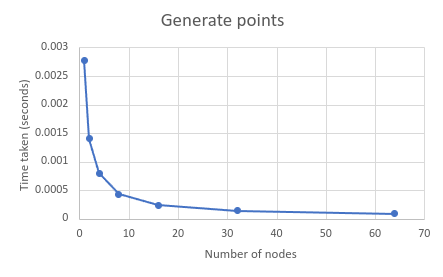
\includegraphics[width=\textwidth]{generate-points.png}
\caption{Generating the points}
\label{fig:1}
\end{figure}
\begin{table}[!htb]
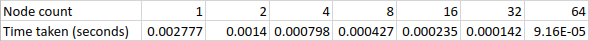
\includegraphics[width=\textwidth]{generate-points-table.png}
\caption{Generating the points}
\label{tab:1}
\end{table}

Figure \ref{fig:1} and table \ref{tab:1} above shows the amount of time taken by each node on
average to generate a portion of the 10000 points by sampling them from the GMM.

\clearpage
\begin{figure}[!htb]
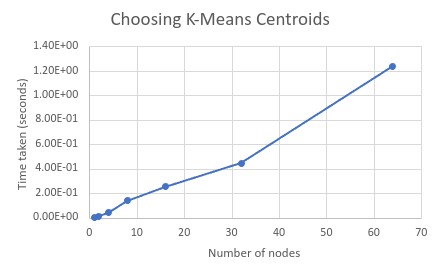
\includegraphics[width=\textwidth]{choose-centroids.png}
\caption{Choosing Centroids for k-means++}
\label{fig:2}
\end{figure}
\begin{table}[!htb]
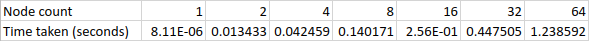
\includegraphics[width=\textwidth]{choose-centroids-table.png}
\caption{Choosing Centroids for k-means++}
\label{tab:2}
\end{table}

Figure \ref{fig:2} and table \ref{tab:2} above shows the amount of time taken by each node on
average to choose the centroids of the clusters with k-means++.

\clearpage
\begin{figure}[!htb]
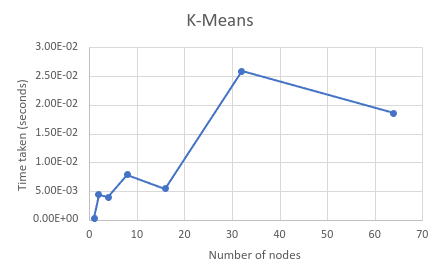
\includegraphics[width=\textwidth]{k-means.png}
\caption{K-Means}
\label{fig:3}
\end{figure}
\begin{table}[!htb]
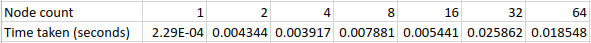
\includegraphics[width=\textwidth]{k-means-table.png}
\caption{K-Means}
\label{tab:3}
\end{table}

Figure \ref{fig:3} and table \ref{tab:3} above shows the amount of time taken by each node on
average to cluster all the points using k-means++.

\clearpage
\begin{figure}[!htb]
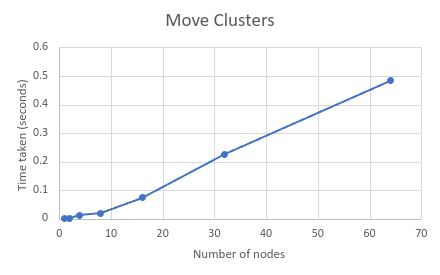
\includegraphics[width=\textwidth]{move-clusters.png}
\caption{Transfer clusters}
\label{fig:4}
\end{figure}
\begin{table}[!htb]
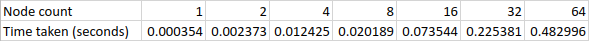
\includegraphics[width=\textwidth]{move-clusters-table.png}
\caption{Transfer clusters}
\label{tab:4}
\end{table}

Figure \ref{fig:4} and table \ref{tab:4} above shows the amount of time taken by each node on
average to transfer the points so that all points of a cluster are stored by a single node.

\clearpage
\begin{figure}[!htb]
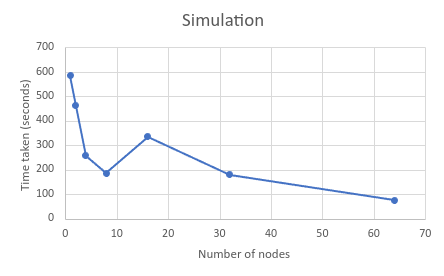
\includegraphics[width=\textwidth]{simulation-time.png}
\caption{Simulation}
\label{fig:5}
\end{figure}
\begin{table}[!htb]
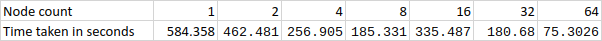
\includegraphics[width=\textwidth]{simulation-time-table.png}
\caption{Simulation}
\label{tab:5}
\end{table}

Figure \ref{fig:5} and table \ref{tab:5} above shows the amount of time taken by each node on
average to perform the N-Body simulation until the sum of distance goes below \(1/2\) of the initial
value. Note that during all runs, the program ran 44 iterations of the simulation before it stopped.

\clearpage
\subsection*{All Process on One Node}
All figures and table shown in this subsection are from running the implementation with all Open MPI
process on a single node but each of them have its own core.

\begin{figure}[!htb]
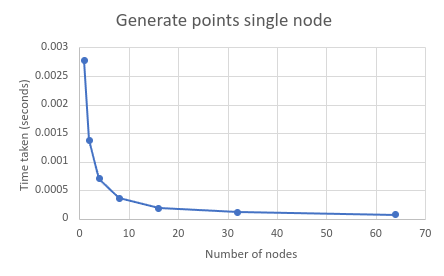
\includegraphics[width=\textwidth]{single-node/generate-points.png}
\caption{Generating the points}
\label{fig:6}
\end{figure}
\begin{table}[!htb]
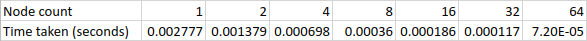
\includegraphics[width=\textwidth]{single-node/generate-points-table.png}
\caption{Generating the points}
\label{tab:6}
\end{table}

Figure \ref{fig:6} and table \ref{tab:6} above shows the amount of time taken by each process on
average to generate a portion of the 10000 points by sampling them from the GMM.

\clearpage
\begin{figure}[!htb]
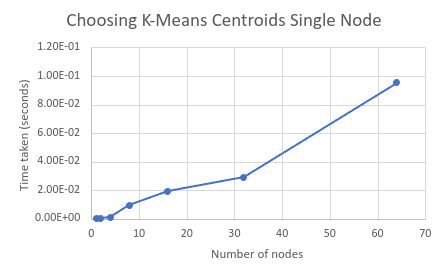
\includegraphics[width=\textwidth]{single-node/choose-centroids.png}
\caption{Choosing Centroids for k-means++}
\label{fig:7}
\end{figure}
\begin{table}[!htb]
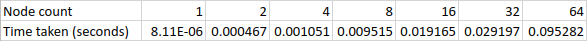
\includegraphics[width=\textwidth]{single-node/choose-centroids-table.png}
\caption{Choosing Centroids for k-means++}
\label{tab:7}
\end{table}

Figure \ref{fig:7} and table \ref{tab:7} above shows the amount of time taken by each process on
average to choose the centroids of the clusters with k-means++.

\clearpage
\begin{figure}[!htb]
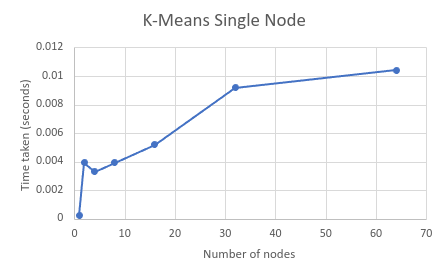
\includegraphics[width=\textwidth]{single-node/k-means.png}
\caption{K-Means}
\label{fig:8}
\end{figure}
\begin{table}[!htb]
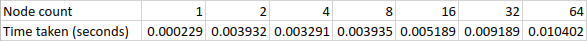
\includegraphics[width=\textwidth]{single-node/k-means-table.png}
\caption{K-Means}
\label{tab:8}
\end{table}

Figure \ref{fig:8} and table \ref{tab:8} above shows the amount of time taken by each process on
average to cluster all the points using k-means++.

\clearpage
\begin{figure}[!htb]
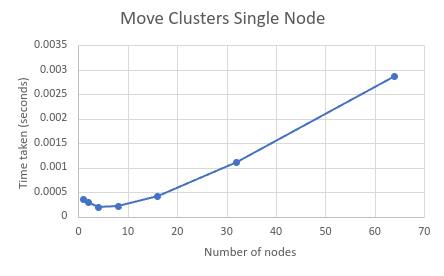
\includegraphics[width=\textwidth]{single-node/move-clusters.png}
\caption{Transfer clusters}
\label{fig:9}
\end{figure}
\begin{table}[!htb]
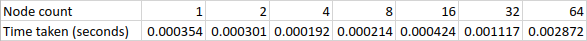
\includegraphics[width=\textwidth]{single-node/move-clusters-table.png}
\caption{Transfer clusters}
\label{tab:9}
\end{table}

Figure \ref{fig:9} and table \ref{tab:9} above shows the amount of time taken by each process on
average to transfer the points so that all points of a cluster are stored by a single process.

\clearpage
\begin{figure}[!htb]
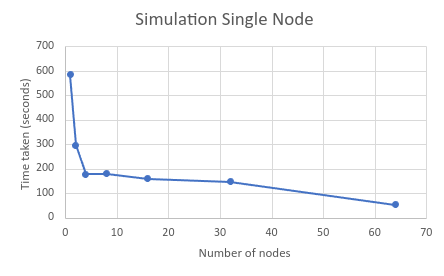
\includegraphics[width=\textwidth]{single-node/simulation.png}
\caption{Simulation}
\label{fig:10}
\end{figure}
\begin{table}[!htb]
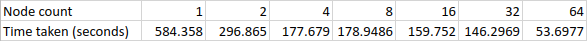
\includegraphics[width=\textwidth]{single-node/simulation-table.png}
\caption{Simulation}
\label{tab:10}
\end{table}

Figure \ref{fig:10} and table \ref{tab:10} above shows the amount of time taken by each process on
average to perform the N-Body simulation until the sum of distance goes below \(1/2\) of the initial
value. Note that during all runs, the program ran 44 iterations of the simulation before it stopped.

\section*{Analysis \& Discussion}
As we can see in figure \ref{fig:1}, table \ref{tab:1}, figure \ref{fig:6} and table \ref{tab:6},
the amount of time it takes for all the points to be sampled from the GMM are roughly inversely
proportional to the number of processes. This is because the task of generating all points is an
embarrassingly parallel problem in the sense that there are no dependency or need for communication
between the tasks of sampling points from GMM components. There are also no differences between the
time taken when all processes are running on a single node and when all processes are running on
separate nodes. This is because there are no communication between them hence the effect of changing
communication speed does not affect their runtime.

As we can see in figure \ref{fig:2}, table \ref{tab:2}, figure \ref{fig:7} and table \ref{tab:7},
the amount of time it takes to choose all centroids for k-means++ increase proportionally with the
amount of process. Because the number of centroids that needs to be generated are proportional (in
fact identical) with the amount of processes, the total amount of time needed to generate all
centroids are proportional to the square of the number of processes. This is expected because in the
implementation, before ever new center is chosen, distances from every point to every center is
recalculated, leading to a time complexity of \(O(n^2)\) for choosing centroids where n is the
number of clusters. The implementation could be sped up by only recalculating the distance between
every point and the newly computed centers.

Comparing between the runtime of choosing centroids for one process per node in figure \ref{fig:2}
and table \ref{tab:2} and on all process on one node in figure \ref{fig:7} and table \ref{tab:7}, we
can see that having all process run on one node reduces the runtime by roughly 10-fold. This shows
that the communication time dominates when all processes are running on separate node. This means
the implementation of choosing centroids might be sped up significantly by doing all the computation
on a single node.

As we can see in figure \ref{fig:3}, table \ref{tab:3}, figure \ref{fig:8} and table \ref{tab:8},
the time taken to cluster the points via k-means does not show clear relationships with the number
of nodes. One of the reasons of this could be that the amount of iteration needed for k-means to
converse fluctuate as the number of cluster changes. While this explains the fluctuation of the run
time for both of each process on a separate node and all processes on a single node separately. It
does not explain the differences between the shape of figure \ref{fig:3} and figure \ref{fig:8}.
More specifically, it is unclear why 8 clusters takes longer than 16 clusters on one process per
node but slightly shorter than 16 clusters on all process on one node. The only possible explanation
for that is noise. Regardless, in both one process per node and all process on one node scenarios,
the runtime for number of clusters being 2, 8 and 16 are all slightly higher than it would be if
the runtime is linearly proportional to the number of clusters.

Comparing between the runtime of k-means clustering on one process per node in figure \ref{fig:3}
and table \ref{tab:3} and on all process on one node in figure \ref{fig:8} and table \ref{tab:8}, we
can see that they are always within two factors of each other. This shows that the runtime are
relatively not as dominated by communication overhead as the runtime for choosing centroids.

As we can see in figure \ref{fig:4}, table \ref{tab:4}, figure \ref{fig:9} and table \ref{tab:9},
the amount of time taken to move all points to their respective clusters are roughly proportional to
number of clusters. Theoretically, we'd expect the number of points that needs to be transferred to
another process being \(10000 \times \frac{n-1}{n}\) where n is the number of clusters. This means
that the amount of data needed to be sent from one process to another should be similar between 32
clusters and 64 clusters. However, in reality with 64 processes it takes almost double amount of
time to transfer the points. This means that the amount of time taken to transfer the points is
dominated by the overhead for each message that needs to be sent and the size of the messages
doesn't affect the runtime very much. This also mean that the benefit in reduced communication cost
that comes from computing the partial tree might be insignificant as computing the partial tree only
reduces the size of the messages needed to be sent to other processes during the simulation and does
not reduce the number of messages.

Comparing between the runtime of k-means clustering on one process per node in figure \ref{fig:4}
and table \ref{tab:4} and on all process on one node in figure \ref{fig:9} and table \ref{tab:9}, we
can see that it takes roughly 200 times longer when each process is on a separate node. This shows
that the runtime is dominated by communication cost. It also shows that the communication cost is at
least 200 times higher when the processes are on different nodes.

As we can see in figure \ref{fig:5}, table \ref{tab:5}, figure \ref{fig:10} and table \ref{tab:10},
ignoring the jump in runtime for when each process is on a separate node between 8 processes and 16
processes, the runtime of the N-Body simulation is roughly inversely proportional to the number of
processes. This shows that our parallelization technique is successful in reducing the overall
runtime. It also shows a practically near optimal parallelization.

The reason for the jump in runtime for when each process is on a separate node between 8 processes
and 16 processes could be because spartan included some nodes with high communication cost with the
rest of the node in jobs that require 16 or more nodes. If we look at the runtime for 1 to 8 nodes
and the runtime for 16 to 64 nodes separately, they're still mostly inversely proportional to the
number of processes.

We can see a similar jump in runtime for when all processes are on the same node, although it is
much less significant. This could be because that the processes have to be on different sockets for
higher number of processes (a spartan node is made up of 4 18 cores sockets) hence increasing the
communication time between them.

Comparing between the runtime for N-Body simulation on one process per node in figure \ref{fig:5}
and table \ref{tab:5} and on all processes on the same node in figure \ref{fig:10} and table
\ref{tab:10}, we can see that they're within a factor of 2 of each other. This shows that the
runtime of the N-Body simulation is mostly made up of computing cost instead of communication cost.

If we increase the number of processes to a much larger number, the runtime of the N-Body simulation
should continue to decrease in an inversely proportional manner as the runtime is mostly dominated
by computing cost instead of communication cost.

\end{document}
